% For a single appendix
\chapter{Technology Used}  % This will appear as "Appendix A: Title"
% For multiple appendices
\section{Programming Language - TypeScript}
TypeScript \cite{microsoft2024typescript}, developed by Microsoft, is a superset of JavaScript that introduces a powerful static type system. This enhancement allows developers to catch errors early in the development process and provides a superior coding experience through IntelliSense and code completion features.

\begin{figure}[H]
    \centering
    
\includegraphics[width=0.6\textwidth]{root/typescript.png}
    \caption{TypeScript}
\end{figure}

Key features of TypeScript that benefit our development include:
\begin{itemize}
    \item A static typing system that enables clear data type definitions, along with Interfaces and Types for more structured code organization
    \item Generics and Decorators that expand code reusability and extensibility capabilities
    \item Comprehensive support for Object-Oriented Programming principles, including inheritance, interfaces, and abstract classes
\end{itemize}
\paragraph{}These features make TypeScript an ideal choice for our project, as it enhances code reliability and maintainability while providing robust development tools. The strong typing system helps prevent common JavaScript runtime errors by catching them during development, while the OOP support enables us to create well-structured, scalable applications.

\subsection{NextJs Framework}
\begin{figure}[H]
    \centering
    
\includegraphics[width=0.7\textwidth]{root/react.png}
    \caption{NextJs}
\end{figure}
NextJS\cite{nextjs-docs} is a React framework for building high-quality, fast fullstack web applications. What sets it apart from plain React lies in its capabilities:

\begin{itemize}
\item Server-side Rendering (SSR) and Static Site Generation (SSG) optimize SEO and performance, which is difficult to achieve with vanilla React projects
\item App Router based on file system simplifies routing and application structure organization
\item Integrated API Routes enable building full-stack applications within a single project
\end{itemize}

These features make NextJS an ideal choice for modern web development, allowing developers to create high-performance, SEO-friendly applications without the complexities typically associated with setting up server-side rendering or API routes in standard React applications. The framework's file-based routing system also significantly reduces the boilerplate code needed for navigation and page structure, making development more efficient and maintainable.

The built-in optimization features and server-side capabilities of NextJS address many of the limitations of client-side React applications, particularly in areas of performance, SEO, and initial page load times. This makes it particularly valuable for production-grade applications that need to maintain high performance while scaling.
\subsection{CSS Framework - Tailwind CSS}
\begin{figure}[H]
    \centering
    
\includegraphics[width=0.8\textwidth]{root/tallwindcss.png}
    \caption{Tailwind CSS}
\end{figure}
TailwindCSS represents a utility-first approach to CSS, enabling rapid and consistent interface development. This framework provides a pre-defined utility classes system, along with a JIT (Just-In-Time) compiler that optimizes file size. The main advantages of TailwindCSS include rapid development speed, easy maintenance, and excellent scalability.

The recently introduced Tailwind v4 brings even more significant improvements \cite{tailwindcss-docs}. Performance has been dramatically enhanced, with build speeds up to 5 times faster than previous versions. The key enhancements include:

\begin{itemize}
\item Performance Optimization: Full builds in the new engine are up to 5x faster, and incremental builds are over 100x faster, measured in microseconds
\item Unified Toolchain: Built-in import handling, vendor prefixing, and syntax transforms, with no additional tooling required
\item CSS-first Configuration: A reimagined developer experience where you can customize and extend the framework directly in CSS instead of using a JavaScript configuration file
\item Modern Web Features: Built on native cascade layers, wide-gamut colors, and including first-class support for modern CSS features like container queries, @starting-style, popovers, and more
\end{itemize}

These improvements significantly enhance the development experience, making it easier and faster to build modern web applications while maintaining the framework's core principles of utility-first CSS. The shift to CSS-first configuration and improved build performance makes Tailwind v4 an even more powerful tool for web development.


\section{UI Library}  % Becomes "Appendix B: Second Appendix Title"
\subsection{Shadcn/ui}
\begin{figure}[H]
    \centering
    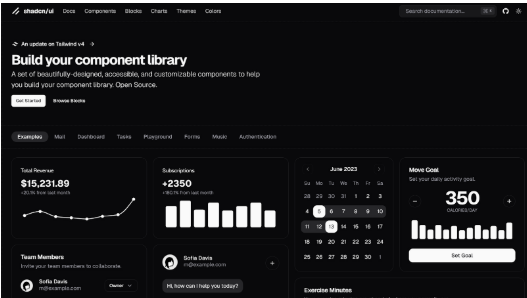
\includegraphics[width=0.8\textwidth]{root/shad.png}
    \caption{Tailwind CSS}
\end{figure}
Shadcn/ui \cite{shadcnui} is a component library featuring modern and aesthetically pleasing interfaces. At its core, Shadcn is built on RadixUI but has been modified to focus on accessibility and customization capabilities. The library is particularly suitable for projects requiring:

\begin{itemize}
\item Components with high accessibility standards and easy customization options
\item Complete source code control
\item Comprehensive TypeScript support
\end{itemize}

Additionally, Shadcn provides Blocks - pre-built code blocks for common functionalities such as Login forms, Dashboards, etc. These blocks come with various layout options and are ready to use, enabling developers to quickly implement them in their projects.

Key advantages of using Shadcn/ui include:

\begin{itemize}
\item High-quality, reusable components that maintain consistency across applications
\item A "copy-paste" approach that gives developers full control over the code
\item Strong integration with modern development tools and frameworks
\item Pre-built UI blocks that accelerate development of common features
\item Extensive styling options through Tailwind CSS integration
\end{itemize}

The library's focus on accessibility and customization, combined with its pre-built blocks, makes it an excellent choice for developers looking to build professional, user-friendly interfaces while maintaining development efficiency.
\subsection{React Flow ( XYFLow )}
\begin{figure}[H]
    \centering
    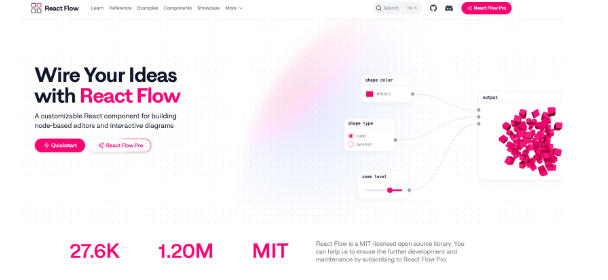
\includegraphics[width=0.8\textwidth]{figures/reactxy.png}
    \caption{React Flow}
\end{figure}
React Flow is a specialized library for building node-based interfaces. This library provides a simple yet powerful API for creating interactive diagrams, workflows, and node-based editors. React Flow stands out with its efficient handling of large graphs, support for custom nodes, and interactive features such as zoom, pan, and events handling.

Key features that make React Flow powerful \cite{reactflow}:

\begin{itemize}
\item Efficient rendering of complex node-based diagrams
\item Fully customizable nodes and edges
\item Comprehensive interaction capabilities
\item Seamless integration with React and TypeScript
\item Built-in support for common graph operations
\end{itemize}

\chapter{Project Architecture} 

These technology stacks combine to create a powerful ecosystem for modern web development. Each component serves a specific purpose:

\begin{itemize}
\item TypeScript ensures type safety and improved developer experience
\item Next.js provides a comprehensive framework for full-stack applications
\item TailwindCSS simplifies styling with its utility-first approach
\item Shadcn/ui delivers high-quality, accessible components
\item React Flow enables complex node-based interface development
\end{itemize}

Together, these technologies form a robust and popular stack that's particularly well-suited for enterprise projects requiring high maintainability and scalability. The integration between these tools creates a seamless development experience, allowing teams to build sophisticated web applications efficiently while maintaining code quality and performance.
\section{Root Directory}
\begin{figure}[H]
    \centering
    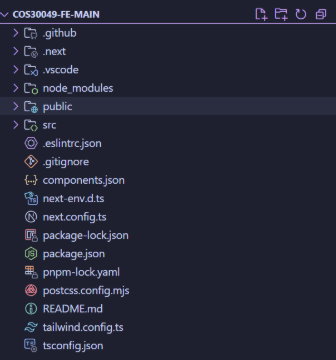
\includegraphics[width=0.55\textwidth]{figures/architecture.png}
    \caption{Architecture}
\end{figure}
Contains essential configuration files for the project:

\begin{itemize}
\item next.config.ts: Configuration for Next.js framework
\item tailwind.config.ts: Configuration for TailwindCSS
\item tsconfig.json: TypeScript configuration file
\item package.json: Manages project dependencies and scripts
\end{itemize}

These configuration files are crucial for setting up the development environment and maintaining consistency across the project.
\subsection{Public}
\begin{figure}[H]
    \centering
    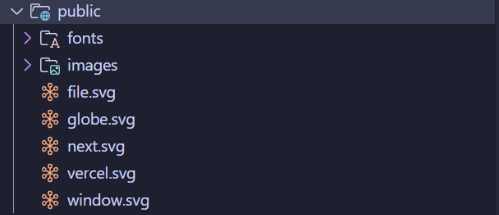
\includegraphics[width=0.6\textwidth, keepaspectratio]{figures/Public.png}
    \caption{Public}
\end{figure}
Manages static resources of the application:

\begin{itemize}
\item fonts: Typography fonts (Figtree, Poppins)
\item images: Images organized by modules
\item SVG assets and other resources
\end{itemize}
\subsection{Src}
\begin{figure}[H]
    \centering
    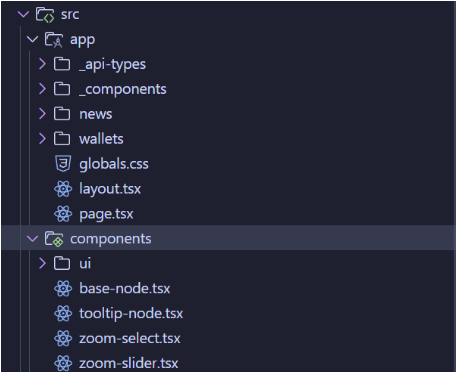
\includegraphics[width=0.55\textwidth]{figures/src.png}
    \caption{Src}
\end{figure}
Main directory containing application source code, organized into modules:

\begin{itemize}
\item app: Components and pages following Next.js App Router structure
    \begin{itemize}
    \item \_api-types: API type definitions
    \item \_components: Shared components for landing page
    \item news: News module
    \item wallets: Wallet management module, including details and transactions
    \end{itemize}
\item components: Reusable components
    \begin{itemize}
    \item ui: Basic components from Shadcn/ui
    \item Base components for common functions
    \end{itemize}
\item lib: Common utilities and types
    \begin{itemize}
    \item utils.ts: Utility functions
    \item types.ts: Shared type definitions
    \item typegen.ts: Automatic type generation tool
    \end{itemize}

\end{itemize}
